% Intended LaTeX compiler: pdflatex
\documentclass[12pt]{article}
\usepackage[utf8]{inputenc}
\usepackage[T1]{fontenc}
\usepackage{graphicx}
\usepackage{longtable}
\usepackage{amsmath}
\usepackage{amssymb}
\usepackage{hyperref}
\usepackage[english]{babel}
\usepackage{url}
\usepackage{sbc-template}
\sloppy
\date{}
\title{``Wait, Is This About Me?'': Encoders, LLMs and System One Models on Conversational Context, Irony and Target-Directed Sentiment}
\hypersetup{
 pdfauthor={Rayan Raddatz de Matos, Eduardo Magnus Lazuta},
 pdftitle={Wait, Is This About Me? Encoders, LLMs and System One Models on Conversational Context, Irony and Target-Directed Sentiment},
 pdfkeywords={},
 pdfsubject={},
 pdfcreator={Emacs 30.2 (Org mode 9.7.11)},
 pdflang={English}}
\begin{document}

\makeatletter
\let\orgtitle\@title
\makeatother

\title{\orgtitle}

\author{
   Rayan Raddatz de Matos\inst{1},
   Eduardo Magnus Lazuta\inst{1}}

\address{
   Instituto de Informática -- Universidade Federal do Rio Grande do Sul (UFRGS)\\
   Caixa Postal 15.064 -- 91.501-970 -- Porto Alegre -- RS -- Brazil
   \email{rayan.raddatz@inf.ufrgs.br},
   \email{eduardo.lazuta@inf.ufrgs.br}}

\maketitle
\begin{abstract}
Whether a comment is for or against a target often depends on the conversation around it: a reply may never name the brand it is about, and irony may say the opposite of what it means. We ask whether conversational context helps models recover sentiment toward a specific target, and how three model families handle it: pretrained encoders, generative LLMs and the recently released \emph{System One} decision models, which answer typed questions with a probability distribution instead of generated text. We evaluate six models of up to 7B parameters, without fine-tuning, on four English datasets (9,202 items), with isolated text, conversational context and irony. Context does not help consistently: on a paired cohort of 456 MT-CSD items, Qwen3.5-4B gained 7.0 percentage points while DeBERTa-NLI lost 22.6, as models tend to follow the tone of the conversation even when the target comment disagrees with it. The \emph{System One} model Kev-4B was the most accurate on MT-CSD (71.3\%) but also drifted toward the tone of the thread, and no model was well calibrated on ironic items. With irony, most targets are criticized, and part of the apparent success comes from a tendency to answer ``negative'' rather than from recognizing what is meant.
\end{abstract}

\section{Introduction}
\label{sec:orged62fcf}

Sentiment analysis usually treats each text as a self-contained unit. In conversations, however, a comment may not mention its target, and its orientation only becomes clear in light of the previous turns. Irony adds another difficulty: the literal content may diverge from the intent. A classifier can thus do well on isolated examples and still fail when it must integrate context or tell literal praise from criticism.

We compare three model families without fine-tuning: pretrained encoders, generative LLMs and \emph{System One} decision models, on isolated text (T1), with conversational context (T2) and on ironic and non-ironic subsets (T3). The questions guiding the study are: (i) does context improve classification? (ii) does this effect hold for ironic texts? (iii) how does context change predictions per class? and (iv) do \emph{System One} models behave differently in bias and calibration?

Our contributions are a comparison of the three families under a common protocol, a paired analysis of the effect of adding turns, and a demonstration that accuracy alone overestimates performance on imbalanced datasets. The rest of the paper is organized as follows. Section~\ref{sec:org6b495ce} reviews related work. Section~\ref{sec:org46ba3a7} describes our methodology, datasets and models. Section~\ref{sec:org92de641} presents and analyzes the results of our experiments. Lastly, Section~\ref{sec:org5902ce0} concludes the paper.
\section{Related Work}
\label{sec:org6b495ce}

Sentiment toward a specific target is not always the sentiment of the text as a whole. \cite{jiang2011target} showed that about 40\% of the errors of sentiment classifiers on Twitter came from ignoring the target entity. Stance detection makes this gap explicit: in SemEval-2016 \cite{mohammad2016semeval}, the target may not even be mentioned in the text. In conversations, the orientation of a comment is often defined only by the previous turns, and MT-CSD \cite{niu2024challenge} was built to capture this setting by providing the full discussion as context. Even so, the best trained models on it stay below 51\% accuracy.

Irony adds a further layer, since the literal content may point the opposite way of the intended one. \cite{riloff2013sarcasm} characterized the common pattern of positive sentiment followed by a negative situation, and \cite{ghosh2018sarcasm} showed that reading the previous turn also helps to detect sarcasm, a finding that motivated datasets with dialogue context such as MUStARD \cite{castro2019towards}. How irony affects sentiment classification itself has received less attention, but \cite{bhargava2025impact} report that classifiers get only 30\% to 60\% of sarcastic tweets right.

Large language models have since become a common alternative to fine-tuned classifiers. With prompting, they are competitive on simple sentiment tasks but fall behind smaller fine-tuned models on finer-grained ones \cite{zhang2023sentiment}. Beyond accuracy, the reliability of their confidence is also a concern. Modern networks tend to be overconfident \cite{guo2017calibration}, the confidence verbalized by LLMs carries little information \cite{xiong2024can}, and even a sentiment RoBERTa becomes less confident on sarcastic texts \cite{shroff2026ai}. For this reason, we rely on label probabilities rather than on verbalized confidence.

More recently, \emph{System One} models proposed a third path between these families. Jev \cite{typesafe2026jev} introduced discriminative \emph{zero-shot} models that take a text and a typed question and return a distribution over the options without generating text, and open alternatives such as Laya \cite{convai2026laya} and Kev \cite{palmer2026kev} soon followed. The closest work to ours is \cite{rafe2026benchmarking}, which compared \emph{System One} models such as Jev, Laya and Kev against generative LLMs and fine-tuned encoders. A fine-tuned encoder obtained the highest accuracy on most labeled tasks, and Jev was close to calibrated on intent tasks (ECE of about 0.03) but not on social-science tasks such as politeness and conversation derailment (about 0.25), where swapping the order of ``yes'' and ``no'' also changed about half of its answers. Emo-Jev \cite{zhang2026emojev} brought Jev closer to affective tasks, evaluating it on sentiment and sarcasm. Building on these efforts, our work turns to sentiment toward a specific target in conversations. We follow how each family responds as conversational turns are added, look at how predictions shift across classes, and examine ironic subsets in light of class prevalence and calibration.

\section{Methodology}
\label{sec:org46ba3a7}
We compare predictions in three conditions: T1, the isolated target text, T2, the same text with the previous turn or with the available conversation, and T3, the ironic and non-ironic subsets, without context. We train no models: ``\emph{zero-shot}'' only means there was no tuning for our evaluations, not that the models never saw sentiment data in their original training. An MT-CSD example illustrates T1 and T2: the target comment ``Reduces driver fatigue during long trips where it's just hundreds of miles of straight highway'' does not mention Tesla, and in isolation it looks like a general statement, but given the conversation about Autopilot, the reference label is in favor of Tesla.

\subsection{Datasets and models}
We use four English datasets with 9,202 items (Table~\ref{tab:bases}). In MT-CSD, we only use Tesla and SpaceX from the test split. The original labels were mapped to negative, neutral and positive: favorable evaluations as positive, unfavorable ones as negative, and labels without clear polarity as neutral (in Filatova, 1--2 stars are negative, 3 neutral and 4--5 positive). Since the original labels measure emotion, stance and stars, the harmonized classes are an approximation, not equivalent constructs.

\begin{table}[!htb]
\centering
\small
\caption{Datasets, labels and evaluated tasks.}
\label{tab:bases}
\setlength{\tabcolsep}{4pt}
\begin{tabular}{llrll}
\hline
Dataset & Source & Items & Original label & Tasks \\
\hline
MUStARD++ & TV-series conversations & 1,171 & intended emotion & T1, T2, T3 \\
MT-CSD & Reddit, brands & 848 & stance toward brand & T1, T2 \\
Sarcasm\_NLP & Twitter, nuclear power & 5,929 & annotated sentiment & T1, T3 \\
Filatova & Amazon reviews & 1,254 & stars & T1, T3 \\
\hline
\end{tabular}
\end{table}

We chose two models from each family (Table~\ref{tab:modelos}). For the LLMs, we read the probability the model assigns to each label as the next word of the prompt. Since some labels are split into several tokens, we score only their first token, and we checked on 8,030 inputs that this gives the same answer as scoring the full word in every case. The predicted class is the most probable one, and its probability is the confidence. Kev-4B starts from the same base as Qwen3.5-4B, but differs from it in several ways at once: an adapter and decision head, training on sentiment data and a calibration temperature. Differences between the two therefore cannot be attributed to any single one of these factors.

\begin{table}[!htb]
\centering
\small
\caption{Evaluated models and how predictions are obtained.}
\label{tab:modelos}
\setlength{\tabcolsep}{4pt}
\begin{tabular}{lll}
\hline
Model & Family & Prediction extraction \\
\hline
twitter-roberta & Encoder & classification output \\
DeBERTa-NLI & Encoder & one NLI hypothesis per label \\
Qwen3.5-4B, Mistral-7B & Generative LLM & label probability as next token \\
Kev-4B, Laya & \emph{System One} & distribution over the options \\
\hline
\end{tabular}
\end{table}

\subsection{Protocol and metrics}
Context comparisons are paired: the same items in T1 and T2. In MT-CSD, we also run an ablation from \(k=0\) to \(k=4\) turns on a fixed cohort of 456 items with at least four turns, which keeps the composition constant across values of \(k\). These items come from only 13 discussions, so results on this cohort carry high uncertainty. On 785 items, we also contrast the initial post and the immediately preceding comment. We evaluate accuracy, macro F1 and balanced accuracy (mean recall over the three classes): accuracy weighs each example equally, while macro F1 and balanced accuracy weigh classes equally. We report 95\% confidence intervals for paired differences, obtained by bootstrap with 2,000 resamples. In MT-CSD we resample whole discussions, and elsewhere we resample items. To assess the models' own confidence, we use the expected calibration error (ECE, 15 bins) and the share of errors made with confidence \(\geq 0.9\). ECE depends on the binning and on the evaluated data, so it is not a fixed property of a model. We also vary option order (three permutations), label descriptions, the question in Sarcasm\_NLP and the description of the Tesla target. Order sensitivity is the fraction of items with the same answer in all three permutations. Unless stated otherwise, results are the mean over the three orders and differences are given in percentage points (pp).
\section{Results}
\label{sec:org92de641}

\subsection{Prompt variations matter mostly on irony}
Without irony, prompt variations had little effect. Accuracy differed by at most 3 pp across option orders in 12 of 16 model--dataset combinations, and describing Tesla in more detail changed it by at most 3 pp. On ironic items, option order mattered much more, especially for Mistral-7B, the least stable model (63.5\% of answers unchanged across the three orders, against 82.8--87.8\% for the other models). On the ironic MUStARD++ items, its accuracy went from 50.7\% to 10.6\% depending on whether ``negative'' or ``neutral'' came first. Rerunning Mistral-7B with all six possible option orders confirmed that it picks the first listed option about 18 pp more often, which explains why it was the model most affected by the order. Label descriptions changed the share of ``neutral'' answers by about 10 pp, and the main exception outside irony was the question in Sarcasm\_NLP, where Mistral-7B went from 50.3\% with ``the topic'' to 71.1\% with ``nuclear power''. In the remaining results, we report the mean over the three orders.

\subsection{Isolated text (T1): no family dominates}
On isolated text, Qwen3.5-4B led on MUStARD++ (59\%) and Kev-4B on MT-CSD (71\%) (Table~\ref{tab:t1}). These two datasets are the starting point for T2.

\begin{table}[!htb]
\centering
\small
\caption{Accuracy and macro F1 (\%) in T1 on the non-ironic items of MUStARD++ (n=570) and MT-CSD (n=848).}
\label{tab:t1}
\setlength{\tabcolsep}{5pt}
\begin{tabular}{lrrrr}
\hline
 & \multicolumn{2}{c}{MUStARD++} & \multicolumn{2}{c}{MT-CSD} \\
Model & Acc. & F1 & Acc. & F1 \\
\hline
twitter-roberta & 50.7 & 50.9 & 52.5 & 50.4 \\
DeBERTa-NLI & 55.3 & 43.7 & 64.7 & 59.7 \\
Qwen3.5-4B & \textbf{58.6} & \textbf{55.8} & 52.4 & 52.7 \\
Mistral-7B & 54.7 & 53.5 & 62.7 & 59.3 \\
Kev-4B & 51.4 & 50.7 & \textbf{71.3} & \textbf{66.1} \\
Laya & 47.5 & 45.2 & 61.7 & 46.1 \\
\hline
\end{tabular}
\end{table}

\subsection{Conversational context (T2): no uniform improvement}
Adding context produced small, isolated gains and larger losses (Figure~\ref{fig:contexto}). On MT-CSD, Qwen3.5-4B gained 5.4 pp with the previous turn, and Kev-4B lost 1.9 and 7.0 pp with the previous turn and the full conversation. On MUStARD++, differences were generally small (Kev-4B +2.8 pp with the conversation). On the ironic MUStARD++ items, Kev-4B and DeBERTa-NLI gained 6.3 pp (95\% CI: [3.0, 9.5]) and 5.7 pp ([1.8, 9.5]), but started answering ``negative'' more often, which does not show better recognition of irony.

\begin{figure}[!htb]
\centering
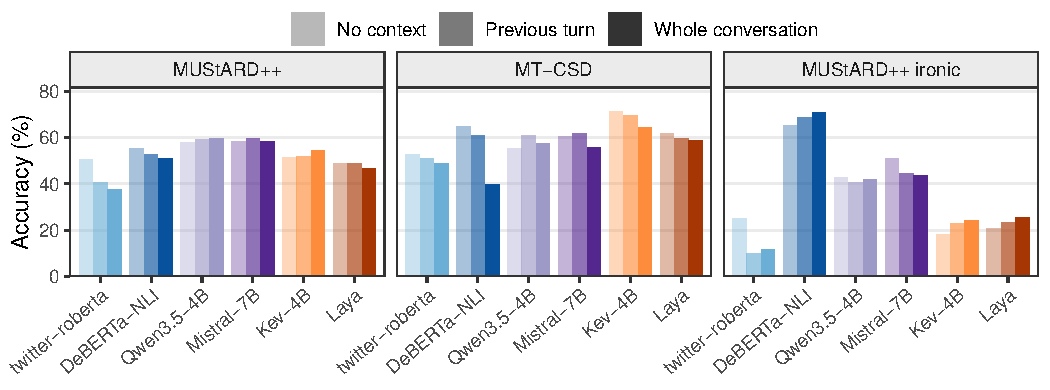
\includegraphics[width=\linewidth]{../base_de_conhecimento/img/fig_contexto-20261126.pdf}
\caption{Accuracy with isolated text, previous turn and full conversation on the tasks with context.}
\label{fig:contexto}
\end{figure}

On the fixed cohort of 456 MT-CSD items (Figure~\ref{fig:turnos}), from \(k=0\) to \(k=4\), Qwen3.5-4B went from 50.9\% to 57.9\% (+7.0 pp, 95\% CI: [3.1, 10.6]), with the whole gain already at \(k=1\), and DeBERTa-NLI dropped from 68.6\% to 46.1\% (-22.6 pp, [-31.6, -13.8]). These are the only two changes at \(k=4\) whose intervals exclude zero. Kev-4B lost 5.6 pp ([-9.8, 0.0]), a borderline drop, while the losses of twitter-roberta (5.0 pp, [-12.3, 1.4]) and Laya (2.5 pp, [-7.8, 4.6]) are within the uncertainty of the cohort. Mistral-7B gained 3.8 pp at \(k=1\) ([1.6, 5.9]) but ended 0.8 pp below its start ([-5.9, 4.2]). Kev-4B kept the highest accuracy and macro F1 at every \(k\). DeBERTa-NLI's macro F1 fell from 61.7\% to 45.5\%, and Qwen's rose from 50.1\% to 56.7\%.

\begin{figure}[!htb]
\centering
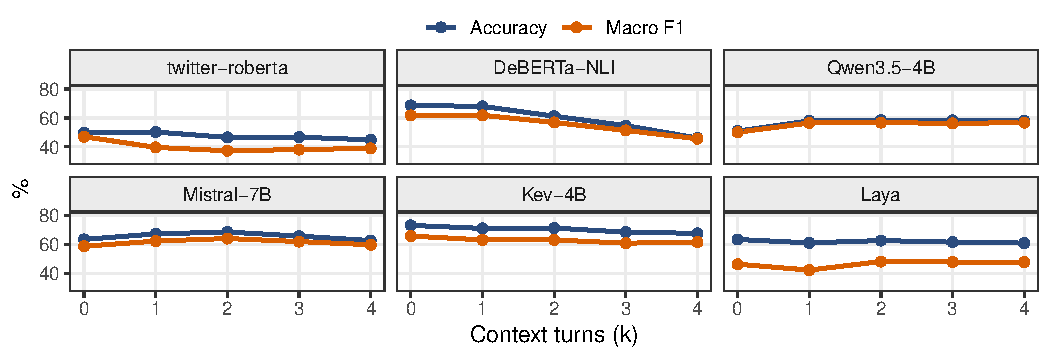
\includegraphics[width=\linewidth]{../base_de_conhecimento/img/fig_turnos-20261126.pdf}
\caption{Accuracy and macro F1 in the ablation from \(k=0\) to \(k=4\) turns, on the same 456 MT-CSD items.}
\label{fig:turnos}
\end{figure}

\subsubsection{Where does the gain of Qwen3.5-4B come from?}
Qwen3.5-4B is the only model whose accuracy clearly rises with context, and its confusion matrices show where this gain comes from (Figure~\ref{fig:qwen-confusao}). Most of it appears with the first turn, which raises the recall of neutral comments from 36\% to 46\% and of ``against'' comments from 81\% to 86\%. The previous comment seems to help the model recognize when the target comment takes no position. After \(k=1\), more turns only trade hits for misses: correct ``against'' predictions rise from 86\% to 93\%, but positives predicted as ``against'' also rise, from 27\% to 31\%, and about 41\% of neutrals remain predicted as ``against'' in every configuration.

\begin{figure}[!htb]
\centering
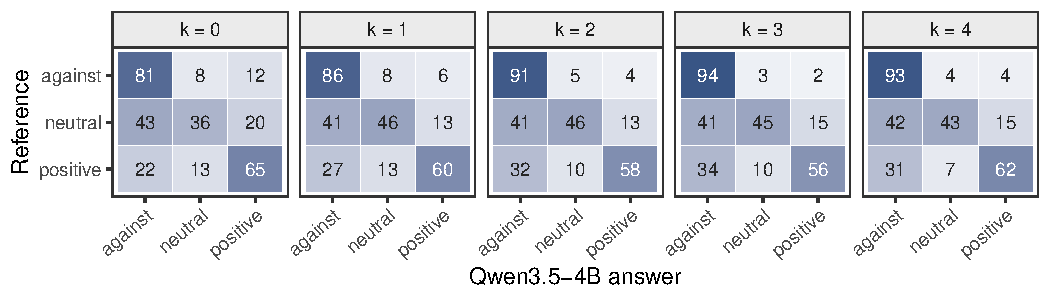
\includegraphics[width=\linewidth]{../base_de_conhecimento/img/fig_qwen_confusao-20261126.pdf}
\caption{Confusion matrices of Qwen3.5-4B on MT-CSD, for \(k=0,\ldots,4\), in percentages per reference class.}
\label{fig:qwen-confusao}
\end{figure}

\subsubsection{Why does more context not help?}
For the other models, more turns did not improve accuracy. Inspecting their errors, we noticed that, as turns were added, many answers seemed to drift toward the overall tone of the conversation, even when the target comment did not share it. To verify this observation, we split the comments into those that agree and those that disagree with the tone of the previous turns (Figure~\ref{fig:tom}). On the 126 disagreeing items, from \(k=0\) to \(k=4\), twitter-roberta followed the tone +39.7 pp more and lost 33.3 pp of accuracy, DeBERTa-NLI +17.5 and -22.2 pp, and Kev-4B +17.2 and -13.2 pp. Qwen3.5-4B, Mistral-7B and Laya changed less (+5.8, +9.3 and +3.2 pp). Context helps when aligned, but induces errors when the stance diverges.

\begin{figure}[!htb]
\centering
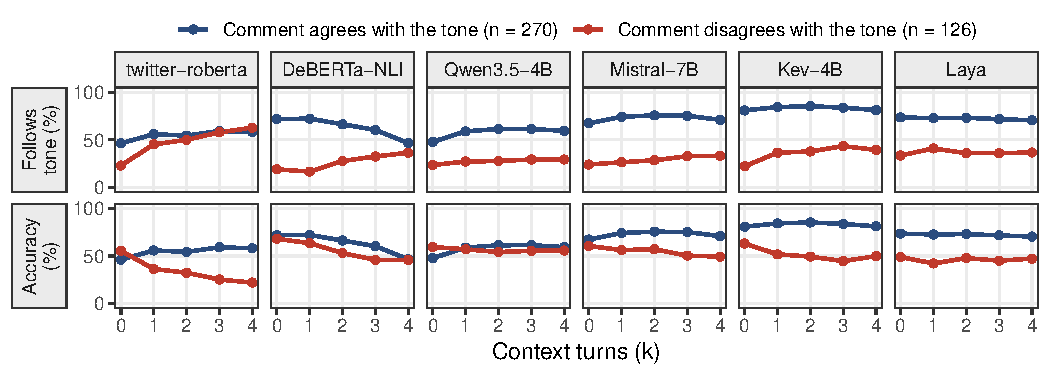
\includegraphics[width=\linewidth]{../base_de_conhecimento/img/fig_tom-20261126.pdf}
\caption{Following the conversation tone and accuracy on agreeing and disagreeing comments, on the MT-CSD ablation items.}
\label{fig:tom}
\end{figure}

DeBERTa-NLI, however, does not fit this pattern: it loses accuracy in both groups, from 71.9\% to 46.7\% on agreeing comments and from 68.3\% to 46.0\% on disagreeing ones (Figure~\ref{fig:tom}), so following the tone alone does not explain its drop. Looking for an explanation, we checked where its answers go as turns are added and found that it stops answering ``neutral'' (Figure~\ref{fig:deberta-neutro}): on the neutral MT-CSD items, its hit rate fell from 72\% without context to 18\% with four turns. With a negative conversation, ``neutral'' fell from 85\% to 15\% and ``against'' rose from 8\% to 73\%, with a positive conversation, ``neutral'' fell from 61\% to 11\%, and even with a neutral conversation it fell from 79\% to 38\%. A plausible, untested explanation is that the neutral hypothesis (``takes no position on Tesla'') loses to the polar ones when the premise contains turns with a stance.

\begin{figure}[!htb]
\centering
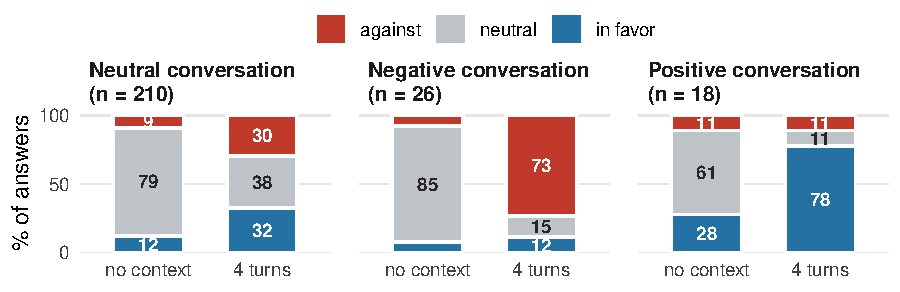
\includegraphics[width=0.86\linewidth]{../base_de_conhecimento/img/fig_deberta-20261126.pdf}
\caption{Neutral predictions of DeBERTa-NLI for neutral MT-CSD comments, by conversation orientation and number of turns.}
\label{fig:deberta-neutro}
\end{figure}

\subsection{Irony (T3): high accuracy may reflect prevalence}
The ironic subsets are imbalanced: in MUStARD++, all are negative, and accuracy equals the proportion of ``negative'' answers, in Sarcasm\_NLP, 87\% are negative, and in Filatova, 66\%, while 86\% of the non-ironic items are positive. Always predicting the majority class already yields 42--86\% accuracy in T1 and 66--100\% in T3 (Figure~\ref{fig:distribuicao-gold} and Table~\ref{tab:balanceada}). With balanced accuracy, Filatova is no longer easy: 82--94\% accuracy becomes 63--76\%. The ranking also changes: on non-ironic Sarcasm\_NLP, Qwen3.5-4B takes the lead (73.8\% against 69.8\% for Kev-4B), and on Filatova, Mistral-7B and Kev-4B are close to 76\%, above Qwen's 65\%. DeBERTa-NLI goes from 41.0\% accuracy to 62.4\% balanced accuracy on Sarcasm\_NLP: it misses the majority neutral class but does better on the others. Balanced accuracy does not solve the scarcity of examples per class, but it prevents prevalence alone from determining the aggregate value.

\begin{figure}[!htb]
\centering
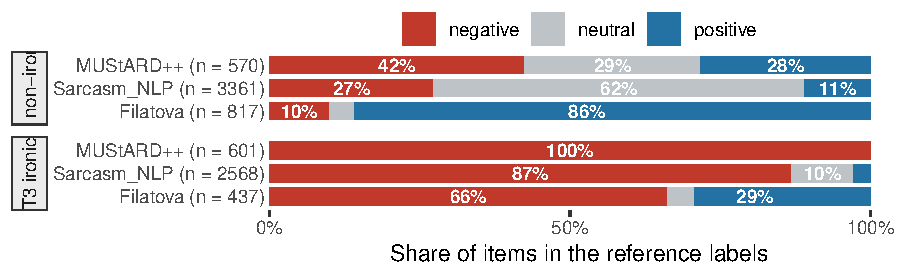
\includegraphics[width=0.86\linewidth]{../base_de_conhecimento/img/fig_gold-20261126.pdf}
\caption{Distribution of reference labels and accuracy of a classifier that always predicts the majority class, by dataset and condition.}
\label{fig:distribuicao-gold}
\end{figure}

\begin{table}[!htb]
\centering
\small
\caption{Balanced accuracy / accuracy (\%) in T1 (non-ironic) and T3 (ironic). Maj.: always predicting the majority class.}
\label{tab:balanceada}
\setlength{\tabcolsep}{3pt}
\resizebox{\linewidth}{!}{%
\begin{tabular}{llccccccc}
\hline
 & Dataset & roberta & DeBERTa & Qwen & Mistral & Kev & Laya & Maj. \\
\hline
T1 & MUStARD++ & 51.7/50.7 & 50.9/55.3 & 56.3/58.6 & 54.9/54.7 & 52.4/51.4 & 48.5/47.5 & 33.3/42.5 \\
T1 & Sarcasm\_NLP & 65.0/70.3 & 62.4/41.0 & 73.8/71.8 & 61.8/71.4 & 69.8/75.4 & 61.6/60.0 & 33.3/61.7 \\
T1 & Filatova & 64.8/81.6 & 63.3/91.8 & 65.2/93.4 & 75.9/92.0 & 75.8/93.6 & 73.1/90.1 & 33.3/85.8 \\
T3 & Sarcasm\_NLP & 42.2/38.0 & 43.1/56.7 & 50.8/64.3 & 50.1/46.1 & 48.5/63.1 & 43.0/29.4 & 33.3/86.8 \\
T3 & Filatova & 61.6/70.9 & 60.0/87.6 & 59.1/85.7 & 65.9/82.5 & 68.3/87.6 & 65.7/80.7 & 33.3/66.1 \\
\hline
\end{tabular}}
\end{table}

\subsubsection{Negative bias analysis}
Each model has a response preference that repeats across datasets (Figure~\ref{fig:distribuicao-pred}): DeBERTa-NLI almost never says ``neutral'' (1--8\%) and answers ``negative'' very often. We measure irony separation as the difference between the frequency of ``negative'' on ironic items and on non-ironic items whose label is not negative (Figure~\ref{fig:ironia}). On Sarcasm\_NLP, separation was 48.9 pp for Kev-4B and 47.8 pp for Qwen3.5-4B, but only 4.7 pp for DeBERTa-NLI (95\% CI: [2.1, 7.6]), which says ``negative'' for 62\% of ironic items and 58\% of non-negative ones. On MUStARD++, all models separated little (7.9--21.5 pp), and accuracy on ironic items was 18--47\%, 18.4 to 27.5 pp below the hit rate on literal negatives: recognizing the negative class is not enough. On Filatova, separation was larger (72--93 pp).

\begin{figure}[!htb]
\centering
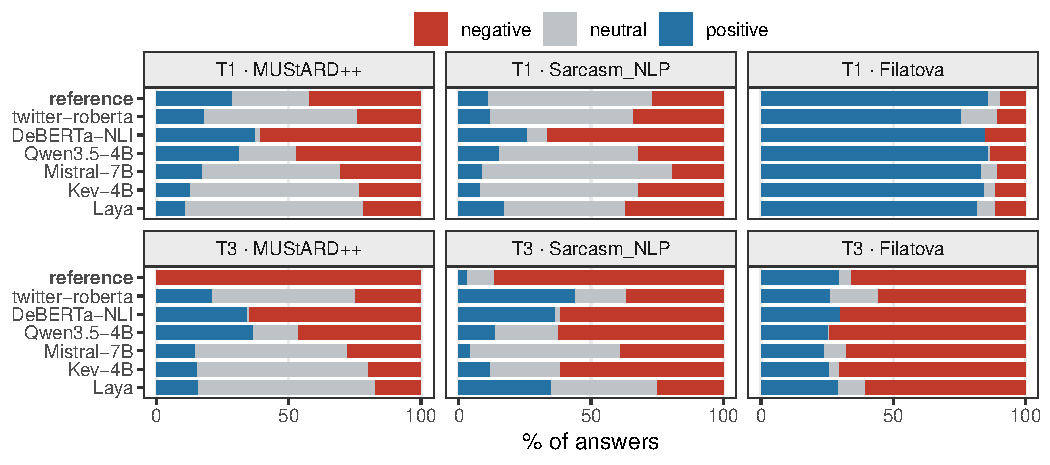
\includegraphics[width=\linewidth]{../base_de_conhecimento/img/fig_distribuicao-20261126.pdf}
\caption{Distribution of predictions and reference labels in T1 and T3.}
\label{fig:distribuicao-pred}
\end{figure}

\begin{figure}[!htb]
\centering
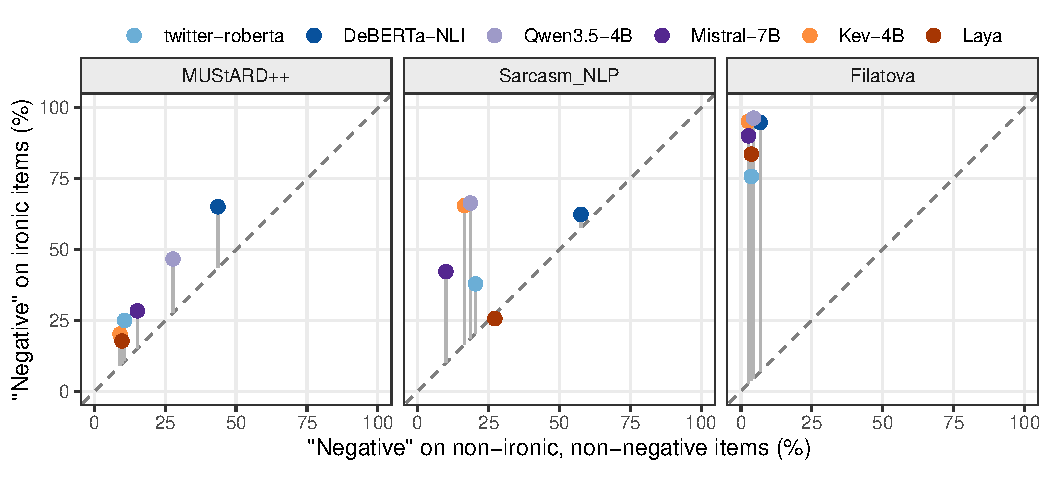
\includegraphics[width=\linewidth]{../base_de_conhecimento/img/fig_ironia-20261126.pdf}
\caption{Proportion of negative answers on ironic items and on non-ironic items whose label is not negative. Distance from the diagonal indicates separation beyond the tendency to answer ``negative''.}
\label{fig:ironia}
\end{figure}

\subsection{Calibration and \emph{System One} models}
Without irony, Kev-4B and Laya had the lowest ECE (0.10--0.16), but they answered ``neutral'' for 65--81\% of items. On ironic items, calibration got worse and no model came close to 0.05, with Laya reaching 0.32. Across the three settings, only 6\% and 3\% of the errors of Kev-4B and Laya were made with confidence \(\geq 0.9\), against 56\% for DeBERTa-NLI and Mistral-7B (Figure~\ref{fig:calibracao}). Part of this caution is simply that Kev-4B and Laya rarely reach a confidence of 0.9. Mistral-7B, in contrast, had a mean confidence of 94\% when correct and 86\% when wrong.

\begin{figure}[!htb]
\centering
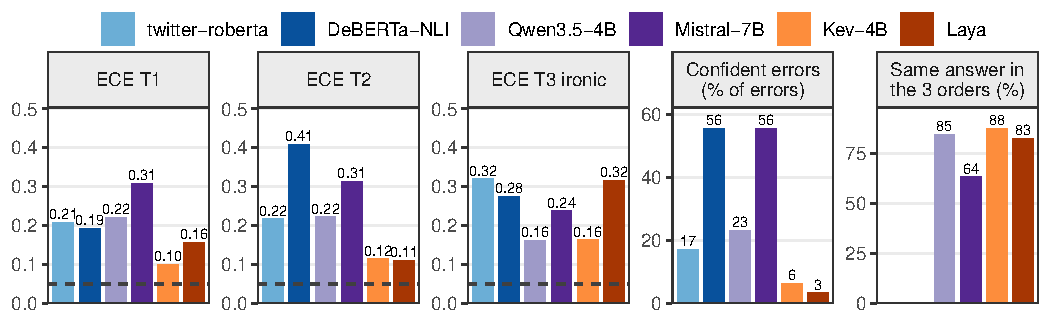
\includegraphics[width=\linewidth]{../base_de_conhecimento/img/fig_calibracao-20261126.pdf}
\caption{ECE in T1, T2 and on ironic items (T3), share of errors made with confidence \(\geq 0.9\) over these three settings, and stability to option order (order v1).}
\label{fig:calibracao}
\end{figure}

Kev-4B and Qwen3.5-4B share the same base (Figure~\ref{fig:qwen-kev}). On MT-CSD, Kev-4B obtained 71.3\% against 55.3\% for Qwen, and its share of neutral answers (65\%) was closer to the 59\% in the reference than Qwen's (29\%). On Sarcasm\_NLP, it also better matched the neutral frequency. On MUStARD++, it predicted neutral for 65\% of items, against 29\% in the reference, and for 68\% of the ironic items, which have no neutrals, where Qwen obtained 42.9\% and Kev 18.0\%. Part of Kev-4B's calibration comes from its temperature (T=2.41): applying it to Qwen reduced its ECE on MUStARD++ from 0.209 to 0.063 without changing the predicted classes. The \emph{System One} models were more cautious on some datasets, not generally superior in competence or calibration.

\begin{figure}[!htb]
\centering
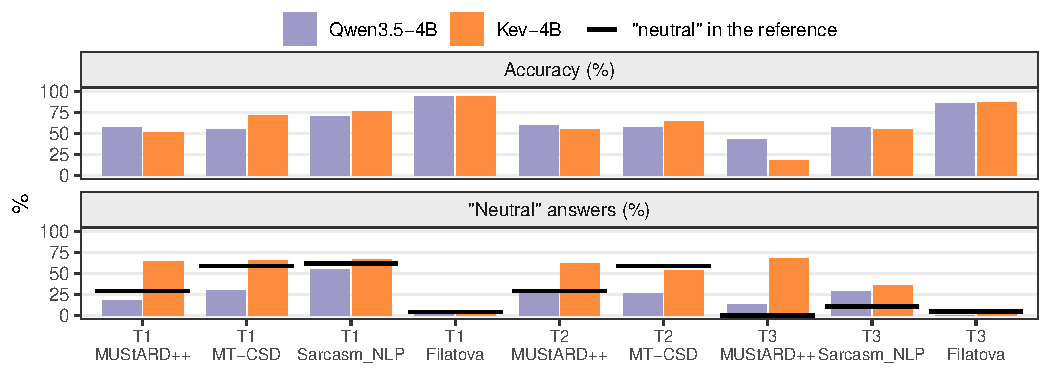
\includegraphics[width=\linewidth]{../base_de_conhecimento/img/fig_qwenkev-20261126.pdf}
\caption{Accuracy and frequency of neutral answers of Qwen3.5-4B and Kev-4B, compared with the reference neutral frequency.}
\label{fig:qwen-kev}
\end{figure}
\section{Conclusion}
\label{sec:org5902ce0}

This study compared six models from three families on sentiment tasks with isolated text, with context and with irony. The answer to the first research question is that context does not help uniformly: on the paired MT-CSD cohort, Qwen3.5-4B gained 7.0 pp and DeBERTa-NLI lost 22.6 pp, while the changes of the other models were small or within the uncertainty of a cohort drawn from only 13 discussions. The per-class analysis suggests that models may follow the conversational tone when it contradicts the target comment, and DeBERTa-NLI's sharp loss of neutrals is consistent with competition between NLI hypotheses, without proving this mechanism.

Regarding irony, accuracy gains must be read in light of the prevalence of negatives and of response bias. Balanced accuracy changed the reading of Filatova and the model ranking, and on Sarcasm\_NLP, DeBERTa-NLI barely separated irony from non-negative examples. On MUStARD++, where all ironic items are negative, getting the class right is not the same as identifying irony. The calibration analysis does not support a general advantage of System One models either: ECE varies with task and temperature, and no model was well calibrated on the ironic subsets. Finally, Mistral-7B's sensitivity to option order and to question wording shows that prompt choices are part of the experimental protocol and must be reported.

There are important limitations: we only evaluated models of up to 7B parameters and English data, we used few prompt formats and no examples, the datasets are imbalanced and their labels represent different constructs, MT-CSD covers only Tesla and SpaceX, without explicit identification of turn authors, and the most controlled ablation uses only 13 discussions. Moreover, differences between models do not isolate effects of architecture or post-training. Future work should include more balanced datasets, additional languages and models, examples in the prompt, speaker identification, explicit separation between question and conversation, and tuning of decision models with context and irony examples.
\section*{Acknowledgments}
The experiments in this work used the PCAD infrastructure, \url{http://gppd-hpc.inf.ufrgs.br}, at INF/UFRGS.

\section*{AI Acknowledgment}
LLMs and AI agents were used in this work to assist in writing and revising the text, including its translation into English, in writing the experiment code, in writing the analysis scripts and producing the figures, in searching the related literature, and in analyzing the data. All outputs were reviewed by the authors, who take full responsibility for the content of this paper.

\bibliographystyle{sbc}
\bibliography{refs}
\end{document}
